\chapter{Subespacios, operadores de proyección y la medición como entrelazamiento}

El teorema de Bell ha dejado dos preguntas pendientes. ¿Qué queda del entrelazamiento cuando uno de los miembros de un par sufre una perturbación, es absorbido o se mide? Y, en concreto, ¿qué convierte una interacción ordinaria en una medición? La respuesta pasa por el álgebra lineal elemental. Las propiedades son subespacios, las probabilidades son valores esperados de proyectores y un aparato de medición es otro sistema cuántico con el que el objeto queda entrelazado.

\section{Motivación inicial: entrelazamiento, localidad y medición}

Supongamos que un singlete se ha separado en dos partes distantes y se mide una de ellas. ¿Debe la teoría cuántica de campos describir un intercambio virtual entre ambas? En el lado lejano no ocurre nada detectable ni llega ningún mensaje utilizable. Se puede rotar localmente un espín mediante un campo magnético y cambiar así la forma concreta del estado conjunto, mientras la cantidad de entrelazamiento permanece fija bajo esa operación local. Más adelante veremos medidas cuantitativas del entrelazamiento; por ahora, el punto es que dos sistemas que ya no interactúan no pueden cambiar el entrelazamiento que comparten por el mero hecho de realizar una operación restringida a uno de los lados.

\begin{classroomqa}\lecturetimestamp{00:00:22}\audiencequestion{¿Una medición de uno de los miembros de un singlete separado por una distancia de tipo espacio requiere algún intercambio virtual con el otro?}\lecturerresponse{En el otro lado no ocurre ningún intercambio detectable. Una operación local puede rotar un factor y alterar la forma en que se escribe el estado conjunto, pero por sí sola no puede enviar un mensaje ni cambiar el entrelazamiento compartido a través de la separación.}\end{classroomqa}

Eso obliga a ampliar la noción de lo que cuenta como el compañero. Si un miembro de un par entrelazado cae en un agujero negro, el otro no deja de estar entrelazado: pasa a estarlo con los grados de libertad del agujero negro y, tras la evaporación, con la radiación emitida. La misma idea no requiere agujeros negros. Se puede dejar caer un miembro de un par entrelazado en una bañera y permitir que se mezcle violentamente con el agua. Aunque su identidad individual se pierda en el estado de muchos cuerpos, la partícula distante sigue entrelazada con la bañera en su conjunto y, con el tiempo, con el vapor que escapa.

No se trata únicamente de la persistencia. También se trata de la reversibilidad. Si una interacción puede crear entrelazamiento, en principio también puede deshacerlo. Es posible desentrelazar los sistemas, pero solo cuando vuelven a entrar en contacto e interactúan de nuevo. Todo lo que puede ocurrir en un sentido puede ocurrir en el otro.

\begin{classroomqa}\lecturetimestamp{00:04:45}\audiencequestion{Si se miden ambos espines de un par entrelazado, ¿siguen entrelazados los electrones? ¿Puede una sola medición desentrelazarlos?}\lecturerresponse{Las mediciones pueden eliminar el entrelazamiento mutuo, y una sola puede bastar. Para entender qué significa esto, en vez de limitarnos a afirmar que ocurre un colapso, debemos describir la observación como una interacción entre el sistema y un aparato de registro.}\end{classroomqa}

Esa pregunta fija el objetivo: relacionar la observación, el colapso del paquete de ondas y el entrelazamiento. Sin embargo, antes de abordarlo necesitamos una explicación más clara de los subespacios y los operadores de proyección, sin recurrir a herramientas más complejas de lo que exige el argumento.

\section{Dimensión, dependencia lineal y bases ortonormales}

Por ahora nos limitaremos a espacios vectoriales de dimensión finita, dotados de bras, kets y un producto interno. Susskind empieza de la manera más elemental posible. No define la dimensión contando las componentes de un vector columna. La define de forma abstracta: la dimensión de un espacio vectorial es el número máximo de vectores linealmente independientes que contiene.

Así, una colección \(\{|v_i\rangle\}\) es linealmente independiente cuando la relación
\begin{equation}
\sum_i c_i |v_i\rangle = 0
\end{equation}
obliga a que todos los coeficientes \(c_i\) sean nulos. De forma equivalente, ninguno de los vectores puede escribirse como combinación lineal de los demás.

Aquí es fundamental no confundir ortogonalidad con independencia. En tres dimensiones puede haber tres vectores que no sean ortogonales en absoluto y, aun así, sean linealmente independientes. Lo que importa es si uno de ellos puede construirse a partir de los otros dos. En cambio, en un plano bidimensional cualquier tercer vector contenido en él debe ser linealmente dependiente de los dos primeros.

\begin{figure}[htbp]\centering
\includegraphics[width=0.56\textwidth]{lecture_06_figure_02.png}\caption{Tres vectores dibujados en la pizarra. En este esquema, la clase distingue la ortogonalidad de la independencia lineal y luego subraya que, en un plano, un tercer vector depende de los dos primeros.}\lectureframe{00:09:35}\end{figure}

\begin{figure}[htbp]\centering
\begin{tikzpicture}[scale=1.2]
\draw[->] (0,0) -- (2.3,0);
\draw[->] (0,0) -- (2.0,2.0);
\draw[->] (0.35,0.95) -- (1.05,1.45);
\fill (0,0) circle (1.2pt);
\end{tikzpicture}\caption{Reconstrucción esquemática del dibujo de la pizarra. El fotograma no determina la relación exacta entre los coeficientes; el punto geométrico es que, en un plano bidimensional, un tercer vector no es independiente.}\end{figure}

Ese es el propósito del esquema. Si el espacio es bidimensional, el número máximo de vectores linealmente independientes es dos. Si es tridimensional, es tres. Más en general, si el espacio tiene dimensión \(d\), dado un producto interno se pueden encontrar \(d\) vectores unitarios mutuamente ortogonales que lo generan. Esos son los vectores de una base. Susskind dice explícitamente que aquí no demostrará ese teorema. Solo le interesa la conclusión: una vez que existe tal base, cualquier vector del espacio puede desarrollarse en ella.

\begin{classroomqa}\lecturetimestamp{00:10:58}\audiencequestion{¿Es el número de grados de libertad espaciales igual a la dimensión del espacio de estados?}\lecturerresponse{No. Una partícula que se mueve en una habitación tiene tres coordenadas espaciales, pero un número enorme de estados cuánticos mutuamente ortogonales. La dimensión del espacio de configuraciones y la dimensión del espacio de Hilbert son conceptos distintos; aquí se usan ejemplos de dimensión finita solo para exponer con claridad la lógica.}\end{classroomqa}

\section{Desarrollo en una base, díadas y resolución de la identidad}

Ahora elijamos una base ortonormal \(\{|n\rangle\}\), con \(n=1,\dots,d\). En este punto, lo escrito en la pizarra es especialmente claro y conciso:

\begin{figure}[htbp]\centering
\includegraphics[width=0.62\textwidth]{lecture_06_figure_03.png}\caption{Base ortonormal y desarrollo de un estado arbitrario.}\lectureframe{00:14:15}\end{figure}

Escribimos
\begin{align}
\langle m|n\rangle &= \delta_{mn}, \\
|\psi\rangle &= \sum_n a_n |n\rangle.
\end{align}
Aquí, \(\delta_{mn}\) es la delta de Kronecker: vale \(1\) cuando \(m=n\) y \(0\) en caso contrario.

\paragraph{Derivación paso a paso.} Los coeficientes se recuperan proyectando sobre la base. Multipliquemos por \(\langle m|\) por la izquierda:
\begin{align}
\langle m|\psi\rangle
  &= \sum_n a_n \langle m|n\rangle \\
  &= \sum_n a_n \delta_{mn} \\
  &= a_m.
\end{align}
Así, los coeficientes son simplemente
\begin{equation}
a_m = \langle m|\psi\rangle.
\end{equation}
El coeficiente es un número complejo ordinario, por lo que se puede poner a cualquiera de los dos lados del ket sin que cambie nada.

Si sustituimos el coeficiente de nuevo en el desarrollo, obtenemos
\begin{equation}
|\psi\rangle = \sum_n |n\rangle \langle n|\psi\rangle.
\end{equation}
Esto sugiere que el objeto \(|n\rangle\langle n|\), y, en general, \(|a\rangle\langle b|\), debe interpretarse como un operador. Ese es precisamente el siguiente paso. Una díada actúa así:
\begin{equation}
\bigl(|a\rangle\langle b|\bigr)|\psi\rangle = \langle b|\psi\rangle\,|a\rangle.
\end{equation}
El bra extrae un número complejo; el ket proporciona la dirección resultante. Esta es la vía elemental de Susskind para pasar de vectores a operadores.

Ahora interpretemos operatorialmente el desarrollo anterior. Puesto que
\begin{equation}
|\psi\rangle = \left(\sum_n |n\rangle\langle n|\right)|\psi\rangle
\end{equation}
para todo \(|\psi\rangle\), el operador entre paréntesis debe ser la identidad:
\begin{equation}
\sum_n |n\rangle\langle n| = I.
\end{equation}
Esto es la resolución de la identidad.

\begin{figure}[htbp]\centering
\includegraphics[width=0.60\textwidth]{lecture_06_figure_07.png}\caption{Resolución de la identidad completa en la pizarra.}\lectureframe{00:18:30}\end{figure}

\begin{classroomqa}\lecturetimestamp{00:18:39}\audiencequestion{¿Es necesario que los vectores de la resolución de la identidad formen una base?}\lecturerresponse{Sí. La derivación requiere tanto la normalización como la ortogonalidad mutua, y la suma debe recorrer una base completa. Una colección arbitraria de vectores no resuelve la identidad.}\end{classroomqa}

El operador identidad es, a su vez, el proyector sobre todo el espacio. Todo vector es un vector propio de \(I\), y todos los valores propios son \(+1\).

\begin{classroomqa}\lecturetimestamp{00:19:14}\audiencequestion{¿La resolución de la identidad afirma que todo vector tiene valor propio uno?}\lecturerresponse{Sí, para el operador identidad. Es un caso excepcional: todo vector es vector propio suyo y \(I|\psi\rangle=|\psi\rangle\) para cualquier estado.}\end{classroomqa}

\section{Las propiedades como subespacios y los operadores de proyección}

Con estas herramientas, la clase introduce su corrección conceptual central. Una propiedad como \(k=\lambda\) no es, en general, un solo vector. Es todo un subespacio.

Sea \(k\) un observable hermítico y supongamos que
\begin{equation}
k|A\rangle = \lambda |A\rangle, \qquad
k|B\rangle = \lambda |B\rangle,
\end{equation}
con \(|A\rangle\) y \(|B\rangle\) linealmente independientes. Entonces, cualquier combinación lineal tiene el mismo valor propio:
\begin{align}
k\bigl(\alpha|A\rangle+\beta|B\rangle\bigr)
  &= \alpha k|A\rangle + \beta k|B\rangle \\
  &= \alpha \lambda |A\rangle + \beta \lambda |B\rangle \\
  &= \lambda\bigl(\alpha|A\rangle+\beta|B\rangle\bigr).
\end{align}
Por tanto, el autoespacio correspondiente a \(\lambda\) es cerrado bajo la suma y la multiplicación por escalares. Es un subespacio vectorial.

El primer ejemplo concreto de la clase es un sistema de dos espines. Los estados
\begin{equation}
|ud\rangle,\qquad |uu\rangle
\end{equation}
tienen distintos valores para el segundo espín, pero el mismo valor para el primero: en ambos casos, el primer espín está hacia arriba. Por eso generan el subespacio en el que \(\sigma_3=+1\) para el primer espín.

\begin{figure}[htbp]\centering
\includegraphics[width=0.46\textwidth]{lecture_06_figure_04.png}\caption{Dos estados de dos espines con el primer espín hacia arriba.}\lectureframe{00:23:27}\end{figure}

Conviene conservar este punto: una propiedad no tiene por qué corresponder a un solo estado. Es toda una colección de estados con el mismo valor propio.

Para evitar la confusión de notación que aparece brevemente en la pizarra, reservaremos las mayúsculas \(A,B,\dots\) para vectores propios concretos y usaremos las minúsculas \(a,b,\dots\) como índices de suma que recorren una base ortonormal del autoespacio. Si \(\{|a\rangle\}\) es una base de ese tipo para el subespacio \(k=\lambda\), el operador de proyección sobre él es
\begin{equation}
\Pi_{k=\lambda}=\sum_a |a\rangle\langle a|.
\end{equation}
No es más que el operador identidad restringido al subespacio. Si \(|\psi\rangle\) ya pertenece a él, el proyector lo devuelve sin modificarlo. Si \(|\psi\rangle\) tiene una componente fuera de él, el proyector elimina la parte ortogonal y conserva solo la componente que pertenece al subespacio.

\section{Postulado de probabilidad, propiedades compatibles y repaso de Bell}

Una vez reinterpretadas las propiedades como subespacios, el postulado de probabilidad adopta su forma más sencilla. Si \(|\psi\rangle\) está normalizado, la probabilidad de que tenga la propiedad \(k=\lambda\) es
\begin{equation}
P(k=\lambda)=\langle\psi|\Pi_{k=\lambda}|\psi\rangle.
\end{equation}

\begin{figure}[htbp]\centering
\includegraphics[width=0.58\textwidth]{lecture_06_figure_05.png}\caption{Proyector sobre el autoespacio de \(k=\lambda\). La disposición en la pizarra prepara el siguiente paso: intercalar el proyector entre \(\langle\psi|\) y \(|\psi\rangle\).}\lectureframe{00:31:09}\end{figure}

Insertamos la forma diádica del proyector:
\begin{align}
P(k=\lambda)
  &= \left\langle \psi \left| \sum_a |a\rangle\langle a| \right| \psi \right\rangle \\
  &= \sum_a \langle\psi|a\rangle\langle a|\psi\rangle \\
  &= \sum_a |\langle a|\psi\rangle|^2.
\end{align}
Esta es exactamente la interpretación de la clase: la probabilidad total de la propiedad es la suma de las probabilidades de todas las formas ortogonales en que puede darse.

Para el primer espín hacia arriba en un sistema de dos espines, el subespacio pertinente está generado por \(|uu\rangle\) y \(|ud\rangle\), así que
\begin{equation}
\Pi_{\sigma_3=+1}=|uu\rangle\langle uu|+|ud\rangle\langle ud|.
\end{equation}
En la notación abreviada de la clase, también se escribe
\begin{equation}
\Pi_{\sigma_3=+1}=\frac{1+\sigma_3}{2},
\end{equation}
omitiendo la identidad que actúa sobre el segundo espín.

\begin{classroomqa}\lecturetimestamp{00:33:04}\audiencequestion{¿Qué diferencia hay entre un observable, una propiedad y un proyector?}\lecturerresponse{El observable es el operador hermítico \(k\). La propiedad \(k=\lambda\) está representada por su autoespacio y significa que, al medir \(k\), el resultado sería con certeza \(\lambda\). El proyector \(\Pi_{k=\lambda}\) aísla ese autoespacio, y su valor esperado da la probabilidad de que la propiedad esté presente.}\end{classroomqa}

\begin{classroomqa}\lecturetimestamp{00:34:07}\audiencequestion{¿Es necesario que los vectores propios degenerados \(A\) y \(B\) ya sean ortogonales, y forman una base de todo el espacio?}\lecturerresponse{Los vectores propios originales no tienen por qué ser ortogonales, pero siempre se puede elegir una base ortonormal dentro de su autoespacio. Esa base solo corresponde a dicho subespacio; hacen falta direcciones ortogonales adicionales para generar el espacio completo. Proyectar sobre cada vector de la base del subespacio y sumar da la proyección sobre el subespacio.}\end{classroomqa}

\begin{classroomqa}\lecturetimestamp{00:35:33}\audiencequestion{¿El símbolo \(a\) en \(k|A\rangle=\lambda|A\rangle\) significa lo mismo que el \(a\) que aparece como índice de suma en el proyector?}\lecturerresponse{No. El primero designa un vector propio concreto, mientras que el índice de la suma recorre todos los vectores de una base ortonormal del autoespacio. Usar notaciones distintas evita confundir una etiqueta fija con un índice mudo de suma.}\end{classroomqa}

\begin{classroomqa}\lecturetimestamp{00:37:15}\audiencequestion{¿Los productos internos de la fórmula del proyector son probabilidades o amplitudes de probabilidad?}\lecturerresponse{Cada \(\langle a|\psi\rangle\) es una amplitud. Al multiplicarla por su conjugado complejo se obtiene una probabilidad, y al sumar esas probabilidades sobre las formas ortogonales de realizar \(k=\lambda\) se obtiene la probabilidad total de la propiedad.}\end{classroomqa}

A continuación, la clase pregunta cómo combinar propiedades. Supongamos que tenemos dos propiedades compatibles, representadas por los proyectores conmutativos \(P_k\) y \(P_\ell\). En el lenguaje de la clase, el enunciado «Y» se representa mediante el producto:
\begin{equation}
\Pi_{k=\lambda\,\wedge\,\ell=\mu}=P_kP_\ell=P_\ell P_k.
\end{equation}
La lógica es sencilla. \(P_k|\psi\rangle\) pertenece al subespacio \(k=\lambda\). Como los operadores conmutan, \(P_\ell P_k|\psi\rangle=P_kP_\ell|\psi\rangle\), así que el mismo vector pertenece también al subespacio \(\ell=\mu\). Por tanto, el producto proyecta sobre la propiedad simultánea. La probabilidad correspondiente es
\begin{equation}
P(k=\lambda,\ell=\mu)=\langle\psi|P_kP_\ell|\psi\rangle.
\end{equation}

Conviene mostrar por separado el primer paso de ese argumento. Para cualquier estado,
\begin{equation}
k\bigl(P_k|\psi\rangle\bigr)=\lambda P_k|\psi\rangle,
\end{equation}
por lo que \(P_k|\psi\rangle\) pertenece al autoespacio \(k=\lambda\). Si \(P_k\) y \(P_\ell\) conmutan, el producto puede escribirse con cualquiera de los dos proyectores a la izquierda y, por tanto, pertenece a ambos subespacios.

\begin{figure}[htbp]\centering
\includegraphics[width=0.44\textwidth]{lecture_06_figure_06.png}\caption{El estado proyectado como vector del autoespacio.}\lectureframe{00:41:57}\end{figure}

\begin{figure}[htbp]\centering
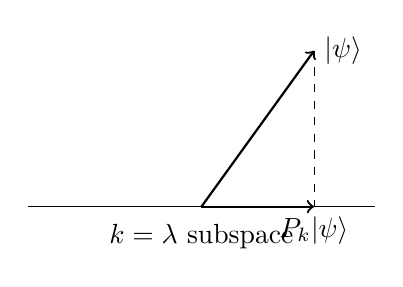
\begin{tikzpicture}[scale=1.1]
\draw (-2,0) -- (2,0);
\draw[->,thick] (0,0) -- (1.3,1.8) node[right] {$|\psi\rangle$};
\draw[dashed] (1.3,1.8) -- (1.3,0);
\draw[->,thick] (0,0) -- (1.3,0) node[below] {$P_k|\psi\rangle$};
\node at (0,-0.35) {$k=\lambda$ subspace};
\end{tikzpicture}\caption{Proyección de un vector arbitrario sobre el autoespacio \(k=\lambda\).}\end{figure}

\begin{figure}[htbp]\centering
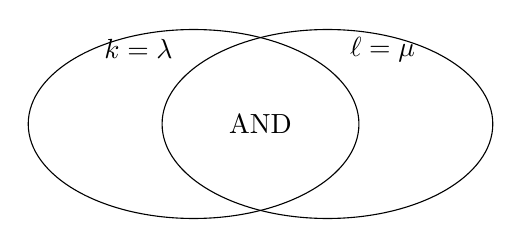
\begin{tikzpicture}[scale=1.0]
\draw (0,0) ellipse (2.1 and 1.2);
\draw (1.7,0) ellipse (2.1 and 1.2);
\node at (-0.7,0.95) {$k=\lambda$};
\node at (2.4,0.95) {$\ell=\mu$};
\node at (0.85,0) {AND};
\end{tikzpicture}\caption{Reconstrucción del dibujo de subespacios que se intersecan y sustenta el enunciado «Y» para proyectores conmutativos.}\end{figure}

\begin{figure}[htbp]\centering
\includegraphics[width=0.66\textwidth]{lecture_06_figure_08.png}\caption{El argumento de la pizarra muestra que los proyectores conmutativos seleccionan el autoespacio simultáneo.}\lectureframe{00:45:20}\end{figure}

\begin{classroomqa}\lecturetimestamp{00:44:42}\audiencequestion{¿La propiedad simultánea es lo mismo que la intersección en la lógica clásica?}\lecturerresponse{Sí. Para proyectores conmutativos, \(P_kP_\ell\) proyecta sobre la intersección de los dos autoespacios. Si la intersección contiene solo el vector nulo, ningún estado no nulo tiene ambas propiedades.}\end{classroomqa}

Para completar el cuadro, el proyector sobre el subespacio compatible de «O» es
\begin{equation}
P_{k\lor\ell}=P_k+P_\ell-P_kP_\ell .
\end{equation}
Cuando las alternativas son mutuamente excluyentes, \(P_kP_\ell=0\), y esto se reduce a la suma \(P_k+P_\ell\). Esta resta es esencial cuando los dos subespacios se solapan, porque su intersección no debe contarse dos veces.

A continuación, se vincula la compatibilidad con ejemplos físicos. En un sistema de dos espines, cualquier componente \(\sigma_i\) del primer espín conmuta con cualquier componente \(\tau_j\) del segundo:
\begin{equation}
[\sigma_i,\tau_j]=0.
\end{equation}
En cambio, las distintas componentes de un mismo espín no conmutan:
\begin{equation}
[\sigma_1,\sigma_3]\neq 0.
\end{equation}
Por eso se puede medir una componente de cada uno de dos espines separados, pero no medir simultáneamente dos componentes distintas de un mismo espín.

\begin{classroomqa}\lecturetimestamp{00:46:12}\audiencequestion{¿Cuáles son ejemplos concretos de observables compatibles?}\lecturerresponse{Todo operador que actúa sobre el primer espín conmuta con cualquier operador que actúa sobre el segundo, porque actúan sobre factores tensoriales distintos. Las componentes de posición \(x,y,z\) forman otra familia compatible. En cambio, dos componentes distintas de un mismo espín, o la posición y su momento conjugado, no conmutan.}\end{classroomqa}

\begin{classroomqa}\lecturetimestamp{00:47:26}\audiencequestion{¿Un subsistema tiene que ser una partícula distinta?}\lecturerresponse{No. Es un conjunto de grados de libertad especificado de manera independiente. Las partículas distintas proporcionan los factores tensoriales más sencillos, pero también se pueden tratar por separado distintos grados de libertad de una sola partícula cuando su estructura de operadores lo permite.}\end{classroomqa}

\begin{classroomqa}\lecturetimestamp{00:48:37}\audiencequestion{Si conmutan tantos operadores de subsistemas distintos, ¿cuál es un ejemplo sencillo de un par incompatible?}\lecturerresponse{Dos componentes de un mismo espín son el ejemplo habitual: \(\sigma_1\) y \(\sigma_3\) no conmutan, así que ningún aparato puede asignarles simultáneamente valores bien definidos. El conmutador matricial no nulo es la prueba algebraica.}\end{classroomqa}

Ahora Susskind vuelve sobre el teorema de Bell. No repite los cálculos de la clase anterior. Reconstruye su lógica en el nuevo lenguaje. La desigualdad clásica, expresada en términos de probabilidades, es
\begin{equation}
P(A\wedge \neg B)+P(B\wedge \neg C)\ge P(A\wedge \neg C).
\end{equation}
Es un teorema de la lógica clásica de conjuntos, no de la mecánica cuántica. En el estado singlete, los espines están antialineados a lo largo de cualquier eje común, así que un enunciado «NO» para el primer espín se puede sustituir por el enunciado positivo correspondiente para el segundo. Esto permite reescribir la desigualdad como un enunciado sobre propiedades conjuntas de un sistema de dos espines.

Si se omiten los operadores identidad que actúan sobre factores no indicados, los proyectores de una sola propiedad que aparecen en la clase son
\begin{equation}
\frac{1+\sigma_3}{2},\qquad
\frac{1+\frac{\tau_1+\tau_3}{\sqrt2}}{2},\qquad
\frac{1+\frac{\sigma_1+\sigma_3}{\sqrt2}}{2},\qquad
\frac{1+\tau_1}{2}.
\end{equation}
Por tanto, los tres proyectores conjuntos pertinentes son
\begin{align}
\Pi_1 &= \frac{1+\sigma_3}{2}\,\frac{1+\frac{\tau_1+\tau_3}{\sqrt2}}{2}, \\
\Pi_2 &= \frac{1+\frac{\sigma_1+\sigma_3}{\sqrt2}}{2}\,\frac{1+\tau_1}{2}, \\
\Pi_3 &= \frac{1+\sigma_3}{2}\,\frac{1+\tau_1}{2}.
\end{align}

\begin{figure}[htbp]\centering
\includegraphics[width=0.68\textwidth]{lecture_06_figure_09.png}\caption{Las tres elecciones de analizadores escritas como productos de proyectores de un espín.}\lectureframe{01:01:45}\end{figure}

En la notación habitual de la pizarra, la clase escribe el singlete, sin normalizar, como
\begin{equation}
|\Psi_{\mathrm{singlet}}\rangle \propto |ud\rangle-|du\rangle.
\end{equation}
Aquí basta con el signo de proporcionalidad. Para la lógica importa el estado mismo y, en particular, el signo relativo, no la normalización global. Al evaluar \(\langle \Pi_1\rangle+\langle \Pi_2\rangle\) frente a \(\langle \Pi_3\rangle\) en el estado singlete, se obtiene la violación derivada en la clase anterior. La conclusión importante es la que Susskind subraya verbalmente: la mecánica cuántica no es la teoría clásica de conjuntos disfrazada.

\begin{classroomqa}\lecturetimestamp{00:52:31}\audiencequestion{Si los estados de espín arriba y espín abajo son ortogonales, ¿significa el signo menos que un ket es el negativo del otro?}\lecturerresponse{No. \(|u\rangle\) y \(|d\rangle\) son vectores distintos y ortogonales. El signo relativo forma parte de una superposición como \(|ud\rangle-|du\rangle\) y puede cambiar sus propiedades físicas; solo es irrelevante un signo global que multiplique el estado completo.}\end{classroomqa}

\begin{classroomqa}\lecturetimestamp{00:53:06}\audiencequestion{¿Se viola la desigualdad de Bell para todo estado cuántico y cualquier elección de propiedades?}\lecturerresponse{No. Muchos estados y muchas elecciones de ejes satisfacen una desigualdad de Bell concreta. La violación depende tanto del estado como de los observables elegidos. Al variar los ángulos intermedio y final, cambia que esta prueba ponga o no de manifiesto las correlaciones no clásicas.}\end{classroomqa}

\begin{classroomqa}\lecturetimestamp{01:02:47}\audiencequestion{¿Qué se puede concluir si un estado concreto viola esta desigualdad de Bell o resulta satisfacerla?}\lecturerresponse{Una violación demuestra que las estadísticas observadas no pueden surgir de la lógica clásica de conjuntos empleada en la derivación. Satisfacer una desigualdad elegida no basta, por sí solo, para que el estado sea clásico, pues otra elección de propiedades puede revelar una violación.}\end{classroomqa}

\section{La localidad después de Bell}

El cálculo con proyectores no es un mero juego simbólico. Imaginemos que preparamos repetidamente pares correlacionados en el estado fundamental singlete, separamos sus dos miembros y dividimos el conjunto preparado de manera idéntica en tres grupos grandes. En el primer grupo se miden las orientaciones \(0^\circ\) y \(45^\circ\); en el segundo, \(45^\circ\) y \(90^\circ\); y en el tercero, \(0^\circ\) y \(90^\circ\). Las frecuencias de los tres grupos permiten estimar las tres probabilidades de la desigualdad.

\begin{classroomqa}\lecturetimestamp{01:04:30}\audiencequestion{¿Qué montaje de laboratorio describen las tres probabilidades de Bell?}\lecturerresponse{Una fuente produce muchos pares entrelazados preparados de manera idéntica y envía sus dos miembros a analizadores separados. Se dividen los pares en tres conjuntos y se usa en cada uno el par correspondiente de direcciones de análisis. El recuento de los resultados conjuntos permite estimar cada probabilidad. Se podría separar mediante un campo una partícula cargada de su antipartícula; en las pruebas de Bell prácticas suelen usarse fotones.}\end{classroomqa}

\begin{classroomqa}\lecturetimestamp{01:08:00}\audiencequestion{La demostración clásica con conjuntos usó una sola población. ¿Cómo pueden ponerla a prueba tres conjuntos medidos por separado?}\lecturerresponse{La desigualdad se refiere tanto a probabilidades como a recuentos. Si las tres muestras proceden del mismo procedimiento de preparación, sus frecuencias relativas estiman las tres distribuciones de probabilidad de un conjunto común. La preparación idéntica es el supuesto indispensable.}\end{classroomqa}

Este repaso de Bell conduce directamente a la inquietud física que aún persiste. Si las correlaciones son reales, ¿por qué no se pueden usar para enviar una señal?

\begin{classroomqa}\lecturetimestamp{01:09:41}\audiencequestion{¿Por qué no se pueden usar las correlaciones entrelazadas para enviar un mensaje más rápido que la luz?}\lecturerresponse{En cada lado se observa por separado una secuencia aleatoria que no se puede controlar. La correlación solo se hace visible cuando se comparan ambos registros mediante un canal clásico ordinario. Sin embargo, una prueba decisiva de Bell organiza las elecciones y las detecciones de modo que ninguna señal luminosa pueda pasar de un lado al otro a tiempo; así se descarta un mecanismo de comunicación local que produzca las estadísticas conjuntas.}\end{classroomqa}

Si transcurre tiempo suficiente para que una señal luminosa viaje entre los aparatos, una correlación no contradice por sí sola la relatividad; quizá solo se haya descubierto una influencia ordinaria inadvertida. El experimento concluyente cierra esa vía de escape. En términos de Bell, toda explicación de variables ocultas que reproduzca las correlaciones debe ser no local, pero la dependencia no local no equivale a un mensaje superlumínico controlable.

\begin{classroomqa}\lecturetimestamp{01:12:18}\audiencequestion{¿Es esencial la conservación del momento angular para este argumento?}\lecturerresponse{No. El espín es un modelo conveniente de dos estados, no un ingrediente inamovible. Cualquier par de sistemas de dos niveles con el estado entrelazado requerido y distintas bases de medición puede mostrar la misma estructura lógica.}\end{classroomqa}

Esta discusión no cierra la clase; despeja el terreno para el siguiente giro. Bell nos ha enseñado que la mecánica cuántica no es lógica clásica, pero ahora la pregunta es otra. ¿Qué es una medición, desde el punto de vista operativo y matemático, y cómo interviene en la interferencia?

\section{Experimento de doble rendija con estados finitos, interferencia y medición como entrelazamiento}

La clase cambia ahora de modelo. Susskind pasa al experimento de doble rendija, pero enseguida lo simplifica y lo convierte en un problema de estados finitos, para poder usar la misma técnica de espacios vectoriales sin introducir toda la maquinaria de la mecánica ondulatoria del continuo. En efecto, dice que sigue siendo el experimento de doble rendija, solo que reducido a un pequeño conjunto de estados de base.

Hay un estado fuente \(|0\rangle\), dos estados de rendija, \(|1\rangle\) y \(|-1\rangle\), y un conjunto de estados de pantalla \(|n\rangle\). Estos estados \(|n\rangle\) son ortonormales porque distintas posiciones de la pantalla corresponden a configuraciones distintas. La clase opta explícitamente por no seguir aquí la normalización con cuidado. Se deja para más adelante la unitariedad. En esta etapa lo que importa es la linealidad.

\begin{figure}[htbp]\centering
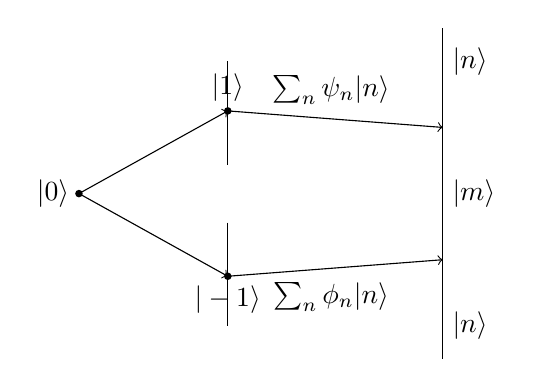
\begin{tikzpicture}[scale=1.05]
\fill (0,0) circle (1.3pt);
\node[left] at (0,0) {$|0\rangle$};

\draw (1.8,1.6) -- (1.8,0.35);
\draw (1.8,-0.35) -- (1.8,-1.6);
\fill (1.8,1) circle (1.3pt);
\fill (1.8,-1) circle (1.3pt);
\node[above] at (1.8,1) {$|1\rangle$};
\node[below] at (1.8,-1) {$|-1\rangle$};

\draw (4.4,2.0) -- (4.4,-2.0);
\node[right] at (4.4,1.6) {$|n\rangle$};
\node[right] at (4.4,0.0) {$|m\rangle$};
\node[right] at (4.4,-1.6) {$|n\rangle$};

\draw[->] (0,0) -- (1.8,1);
\draw[->] (0,0) -- (1.8,-1);
\draw[->] (1.8,1) -- (4.4,0.8);
\draw[->] (1.8,-1) -- (4.4,-0.8);

\node at (3.05,1.25) {$\sum_n \psi_n |n\rangle$};
\node at (3.05,-1.25) {$\sum_n \phi_n |n\rangle$};
\end{tikzpicture}\caption{Versión de estados finitos del experimento de doble rendija: el estado fuente \(|0\rangle\), los dos estados de rendija \(|1\rangle\) y \(|-1\rangle\), y la base de pantalla \(|n\rangle\).}\end{figure}

\begin{figure}[htbp]\centering
\includegraphics[width=0.68\textwidth]{lecture_06_figure_10.png}\caption{La retícula finita de posiciones junto a la regla de evolución lineal \(A\to A'\), \(B\to B'\).}\lectureframe{01:18:00}\end{figure}

Por simetría, el estado fuente evoluciona a una superposición de igual amplitud de los dos estados de rendija:
\begin{equation}
|0\rangle \longrightarrow |1\rangle+|-1\rangle.
\end{equation}
Ahora, dejemos que el estado de la rendija superior evolucione a
\begin{equation}
|1\rangle \longrightarrow \sum_n \psi_n |n\rangle,
\end{equation}
y que el de la rendija inferior evolucione a
\begin{equation}
|-1\rangle \longrightarrow \sum_n \phi_n |n\rangle.
\end{equation}
Las flechas indican evolución temporal, no igualdad de estados en un mismo instante. Por linealidad,
\begin{equation}
|1\rangle+|-1\rangle \longrightarrow \sum_n (\psi_n+\phi_n)|n\rangle.
\end{equation}
Esa es la regla clave. Las amplitudes se suman antes de calcular las probabilidades.

\begin{classroomqa}
\lecturetimestamp{01:21:59}
\audiencequestion{¿Cómo puede el estado de la rendija \(|1\rangle\) transformarse en estados etiquetados también con enteros \(n\)? ¿Son estos kets del mismo lugar y del mismo instante?}
\lecturerresponse{Las etiquetas corresponden a distintos instantes. \(|1\rangle\) representa el electrón en la rendija superior, mientras que los \(|n\rangle\) de la derecha representan posibles posiciones posteriores en la pantalla. La flecha indica evolución temporal, no una igualdad entre configuraciones simultáneas.}
\end{classroomqa}

\begin{classroomqa}
\lecturetimestamp{01:25:30}
\audiencequestion{¿Deben normalizarse las amplitudes y tienen unidades físicas?}
\lecturerresponse{Una evolución completa debe conservar la probabilidad total; eso es la unitariedad. Aquí se omite el factor de normalización común porque solo importan la suma y la cancelación de las amplitudes de los caminos. Los factores de escala pueden restituirse al normalizar el estado.}
\end{classroomqa}

Por tanto, la probabilidad de llegar al punto \(m\) de la pantalla es
\begin{align}
P_m &= |\psi_m+\phi_m|^2 \\
    &= |\psi_m|^2 + |\phi_m|^2 + \psi_m^*\phi_m + \phi_m^*\psi_m.
\end{align}
Los dos primeros términos son los que habría producido el razonamiento clásico. Los dos últimos son los términos de interferencia.

\begin{figure}[htbp]
\centering
\includegraphics[width=0.68\textwidth]{lecture_06_figure_11.png}
\caption{La amplitud en la pantalla y su expansión de cuatro términos para la probabilidad, en la pizarra.}
\lectureframe{01:29:20}
\end{figure}

En el punto simétrico de la pantalla, que llamaremos \(m=0\), la simetría sugiere que \(\psi_0=\phi_0\). Entonces
\begin{equation}
P_0 = |\psi_0+\phi_0|^2 = |2\psi_0|^2 = 4|\psi_0|^2.
\end{equation}
Con ambas rendijas abiertas, la probabilidad en ese punto es cuatro veces la de una sola rendija, no el doble. Es interferencia constructiva.

Ahora introduzcamos un desfase de modo que \(\phi_0=-\psi_0\). Entonces
\begin{equation}
P_0 = |\psi_0-\psi_0|^2 = 0.
\end{equation}
Cada rendija por separado permite llegar a ese punto, pero abrir ambas a la vez puede hacer imposible llegar allí. Es interferencia destructiva. Susskind se detiene expresamente en lo extraño que resulta: a su juicio, es tan desconcertante como el teorema de Bell.

\begin{classroomqa}
\lecturetimestamp{01:33:14}
\audiencequestion{¿Qué ocurre si se cambia el desfasador o la elección de rendija cuando el electrón ya está en vuelo? ¿La otra rendija necesita tiempo para enterarse?}
\lecturerresponse{La respuesta depende de la configuración precisa en el espacio-tiempo y de si el electrón encuentra la parte modificada del aparato. La mecánica cuántica hace evolucionar el estado a través de la configuración real; las probabilidades siguen obteniéndose al sumar las amplitudes pertinentes. Para evaluar las afirmaciones sobre localidad, hay que especificar con precisión una propuesta de elección retardada.}
\end{classroomqa}

Ahora introducimos el aparato. Hay un sistema adicional de dos estados: un espín que inicialmente está en el estado \(|d\rangle\). Si el electrón pasa por la rendija superior, el espín cambia a \(|u\rangle\). Si pasa por la inferior, permanece sin cambios. El estado compuesto inicial es \(|0,d\rangle\), y la primera regla de evolución pasa a ser
\begin{equation}
|0,d\rangle \longrightarrow |1,u\rangle + |-1,d\rangle.
\end{equation}
Esa línea expresa todo el significado de la medición en esta lección. La posición del electrón queda entrelazada con el registro almacenado en el aparato.

\begin{figure}[htbp]
\centering
\includegraphics[width=0.66\textwidth]{lecture_06_figure_12.png}
\caption{El espín del detector correlaciona sus registros de espín arriba y abajo con las dos alternativas de rendija.}
\lectureframe{01:44:10}
\end{figure}

\begin{classroomqa}
\lecturetimestamp{01:40:20}
\audiencequestion{¿Tiene que haber un detector en cada rendija?}
\lecturerresponse{Basta con un detector fiable. Si registra el paso por la rendija superior, un registro sin cambios identifica la alternativa inferior, siempre que todo electrón transmitido tenga que pasar por una de las dos aberturas. Se puede usar un segundo detector, pero añadiría otro subsistema sin cambiar el principio.}
\end{classroomqa}

\begin{classroomqa}
\lecturetimestamp{01:40:51}
\audiencequestion{¿Por qué no decir que el electrón pasa por las dos rendijas?}
\lecturerresponse{Sin un registro del camino, el estado es una superposición coherente y no se dispone de ningún hecho retrospectivo sobre el camino. Con una medición completa de qué camino, el aparato registra una alternativa o la otra en cada ensayo. Lo que persiste a través de ambas alternativas es la amplitud del estado, no dos trayectorias electrónicas observadas por separado.}
\end{classroomqa}

\begin{figure}[htbp]
\centering
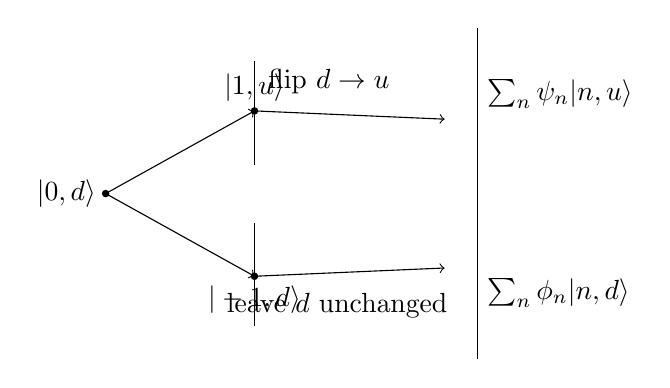
\begin{tikzpicture}[scale=1.05]
\fill (0,0) circle (1.3pt);
\node[left] at (0,0) {$|0,d\rangle$};

\draw (1.8,1.6) -- (1.8,0.35);
\draw (1.8,-0.35) -- (1.8,-1.6);
\fill (1.8,1) circle (1.3pt);
\fill (1.8,-1) circle (1.3pt);
\node[above] at (1.8,1) {$|1,u\rangle$};
\node[below] at (1.8,-1) {$|-1,d\rangle$};

\draw (4.5,2.0) -- (4.5,-2.0);
\node[right] at (4.5,1.2) {$\sum_n \psi_n |n,u\rangle$};
\node[right] at (4.5,-1.2) {$\sum_n \phi_n |n,d\rangle$};

\draw[->] (0,0) -- (1.8,1);
\draw[->] (0,0) -- (1.8,-1);
\draw[->] (1.8,1) -- (4.1,0.9);
\draw[->] (1.8,-1) -- (4.1,-0.9);

\node at (2.7,1.35) {flip \(d\to u\)};
\node at (2.8,-1.35) {leave \(d\) unchanged};
\end{tikzpicture}
\caption{La medición como entrelazamiento con el espín de un detector. El camino superior invierte el espín del aparato; el inferior lo deja intacto.}
\end{figure}

Supongamos, como hace la lección, que no ocurre nada más con el espín durante el trayecto hasta la pantalla. Entonces
\begin{align}
|1,u\rangle &\longrightarrow \sum_n \psi_n |n,u\rangle, \\
|-1,d\rangle &\longrightarrow \sum_n \phi_n |n,d\rangle.
\end{align}
Por tanto, el estado final con ambas rendijas abiertas es
\begin{equation}
|\Psi_{\mathrm{final}}\rangle
  = \sum_n \psi_n |n,u\rangle + \sum_n \phi_n |n,d\rangle.
\end{equation}
No es una superposición de estados de un solo electrón. Es un estado entrelazado del electrón y el aparato.

\begin{figure}[htbp]
\centering
\includegraphics[width=0.68\textwidth]{lecture_06_figure_13.png}
\caption{Las amplitudes de los dos caminos llegan a la pantalla acompañadas de registros ortogonales del aparato.}
\lectureframe{01:47:35}
\end{figure}

La forma más directa de calcular la probabilidad de llegada al punto \(m\) es usar el proyector sobre ese punto en el subsistema del electrón:
\begin{equation}
\Pi_m = |m\rangle\langle m|\otimes I_{\mathrm{spin}}.
\end{equation}
Al aplicar \(\Pi_m\) al estado final se obtiene
\begin{equation}
\Pi_m |\Psi_{\mathrm{final}}\rangle
= |m\rangle\bigl(\psi_m|u\rangle+\phi_m|d\rangle\bigr).
\end{equation}
Así, la probabilidad de llegar a \(m\) es
\begin{align}
P_m
  &= \langle \Psi_{\mathrm{final}}|\Pi_m|\Psi_{\mathrm{final}}\rangle \\
  &= \bigl(\psi_m^*\langle u|+\phi_m^*\langle d|\bigr)
     \bigl(\psi_m|u\rangle+\phi_m|d\rangle\bigr) \\
  &= |\psi_m|^2 + |\phi_m|^2
     + \psi_m^*\phi_m\langle u|d\rangle
     + \phi_m^*\psi_m\langle d|u\rangle.
\end{align}
Pero los estados de registro son ortogonales:
\begin{equation}
\langle u|d\rangle=0.
\end{equation}
Por tanto, los términos cruzados se anulan:
\begin{equation}
P_m = |\psi_m|^2 + |\phi_m|^2.
\end{equation}
Ese es el resultado matemático central de la lección. Una vez registrado qué camino se tomó, desaparece la interferencia y las probabilidades se suman de manera clásica.

\begin{classroomqa}
\lecturetimestamp{01:49:09}
\audiencequestion{¿Cuál es la diferencia entre la superposición \(|1\rangle+|-1\rangle\) y el estado \(|1,u\rangle+|-1,d\rangle\)?}
\lecturerresponse{El primer caso se refiere a un sistema en una combinación lineal de dos posiciones; no hay ningún otro sistema con el que pudiera estar entrelazado. El segundo se refiere a dos sistemas y correlaciona el camino con el espín del detector. Al leer el espín, se obtiene información sobre el camino.}
\end{classroomqa}

\section{Registros ambientales y medición parcial}

Un detector construido deliberadamente no es el único dispositivo que puede registrar el camino. Un átomo cerca de una rendija, el gas residual, una superficie térmica o cualquier otro grado de libertad pueden quedar correlacionados con él. Si sus estados finales son \(|E_1\rangle\) y \(|E_2\rangle\), el estado del camino tiene la forma
\begin{equation}
|\Psi\rangle
=\sum_n\left(\psi_n|n\rangle|E_1\rangle
+\phi_n|n\rangle|E_2\rangle\right).
\end{equation}
Ahora los términos de interferencia quedan multiplicados por el solapamiento \(\langle E_1|E_2\rangle\). Los registros ortogonales hacen que los caminos sean perfectamente distinguibles y eliminan por completo la interferencia. Los registros idénticos dejan \(\langle E_1|E_2\rangle=1\) y la conservan. Un solapamiento intermedio da una visibilidad parcial.

\begin{figure}[htbp]
\centering
\includegraphics[width=0.68\textwidth]{lecture_06_figure_14.png}
\caption{Paquetes de onda ambientales solapados y separados ilustran registros parciales y completos del camino.}
\lectureframe{01:53:40}
\end{figure}

\begin{classroomqa}
\lecturetimestamp{01:50:48}
\audiencequestion{¿Se entrelazaría un átomo corriente cerca de la rendija con el electrón que pasa, aunque nadie lo observe deliberadamente?}
\lecturerresponse{Sí. El verbo pertinente no es conocer, sino correlacionar físicamente. Si el átomo o el gas circundante se alteran lo suficiente como para que su estado posterior permita distinguir el camino, registran información sobre cuál se tomó y suprimen la interferencia. Por eso estos experimentos requieren aislamiento, bajas temperaturas y, a menudo, partículas que interactúan débilmente, como los fotones.}
\end{classroomqa}

El enfriamiento acerca los grados de libertad ambientales a sus estados fundamentales y reduce los registros accidentales. Una brecha energética también ayuda: si la partícula incidente no puede aportar la energía mínima de excitación, quizá el entorno no pueda retener información sobre el camino. En cambio, las partículas cargadas pueden perturbar la materia cercana mediante sus campos eléctricos, lo que hace especialmente exigentes los experimentos de interferencia con electrones.

\begin{classroomqa}
\lecturetimestamp{01:54:49}
\audiencequestion{¿De verdad se puede obtener un patrón de interferencia con electrones individuales?}
\lecturerresponse{Cada electrón produce un único impacto localizado. Envíe las partículas de una en una, con suficiente separación para que no interactúen, y reúna muchas repeticiones. La distribución de frecuencias acumulada muestra el patrón de interferencia; un solo suceso no es más que un destello.}
\end{classroomqa}

\begin{classroomqa}
\lecturetimestamp{01:55:59}
\audiencequestion{¿La medición destruye el entrelazamiento o lo crea?}
\lecturerresponse{La interacción que determina qué camino se tomó crea entrelazamiento entre el sistema y el aparato, y ese entrelazamiento destruye la interferencia entre las alternativas. Una medición posterior puede correlacionar el aparato con otro sistema y quizá condicionar el estado restante. Por eso siempre hay que especificar cuáles son los dos subsistemas y a qué interferencia se hace referencia.}
\end{classroomqa}

\begin{classroomqa}
\lecturetimestamp{01:57:44}
\audiencequestion{¿Se puede debilitar la interacción para que el aparato obtenga solo información parcial sobre el camino?}
\lecturerresponse{Sí. Una interacción débil puede invertir el espín del detector con solo cierta amplitud, de modo que queden estados de registro no ortogonales. En ese caso, los caminos solo son parcialmente distinguibles y la interferencia se reduce solo en parte. Una medición más intensa implica una mayor distinguibilidad, un entrelazamiento más fuerte con el registro y una menor visibilidad de las franjas.}
\end{classroomqa}

El colapso pertinente aquí es, por tanto, algo concreto: la pérdida de los términos cruzados cuando la información sobre el camino queda depositada en otro sistema. Sin registro, se suman las amplitudes. Con registros perfectamente distinguibles, sus productos internos se anulan y se suman las probabilidades. Entre ambos extremos, la intensidad de la medición y la visibilidad de la interferencia varían de forma continua.
